\section{Aulyardha Anindita | 1174054}
\subsection{Membaca Shapefile dengan PySHP}
\begin{enumerate}
 \item Nomor 1
 \lstinputlisting{src/tugas3/1174054/soal1.py}
 \begin{figure}[H]
  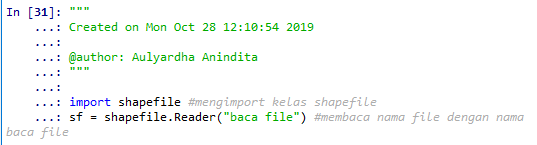
\includegraphics[width=6cm]{figures/Tugas3/1174054/no1.png}
  \centering
  \caption{Gambar Soal 1}
 \end{figure}
 \item Nomor 2
 \lstinputlisting{src/tugas3/1174054/soal2.py}
 \begin{figure}[H]
  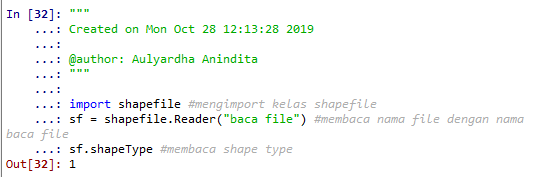
\includegraphics[width=6cm]{figures/Tugas3/1174054/no2.png}
  \centering
  \caption{Gambar Soal 2)}
 \end{figure}
 \item Nomor 3
 \lstinputlisting{src/tugas3/1174054/soal3.py}
 \begin{figure}[H]
  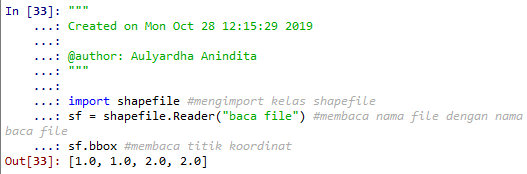
\includegraphics[width=6cm]{figures/Tugas3/1174054/no3.png}
  \centering
  \caption{Gambar Soal 3}
 \end{figure}
 \item Nomor 4
 \lstinputlisting{src/tugas3/1174054/soal4.py}
 \begin{figure}[H]
  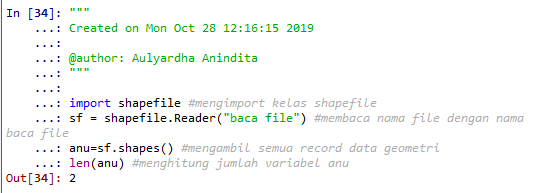
\includegraphics[width=6cm]{figures/Tugas3/1174054/no4.png}
  \centering
  \caption{Gambar Soal 4}
 \end{figure}
 \item Nomor 5
 \lstinputlisting{src/tugas3/1174054/soal5.py}
 \begin{figure}[H]
  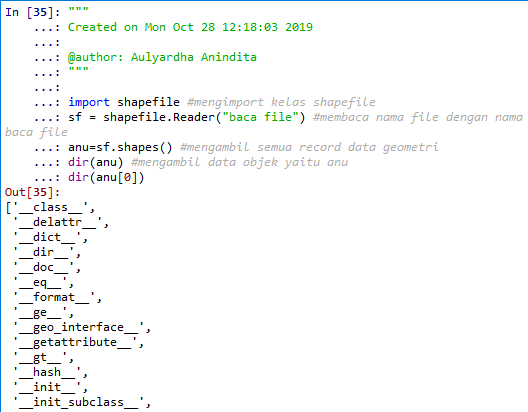
\includegraphics[width=6cm]{figures/Tugas3/1174054/no5.png}
  \centering
  \caption{Gambar Soal 5)}
 \end{figure}
 \item Nomor 6
 \lstinputlisting{src/tugas3/1174054/soal6.py}
 \begin{figure}[H]
  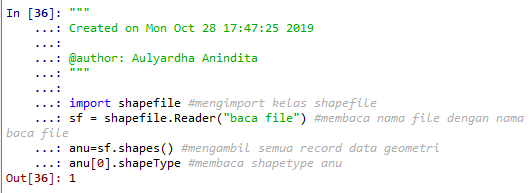
\includegraphics[width=6cm]{figures/Tugas3/1174054/no6.png}
  \centering
  \caption{Gambar Soal 6}
 \end{figure}
 \item Nomor 7
 \lstinputlisting{src/tugas3/1174054/soal7.py}
 \begin{figure}[H]
  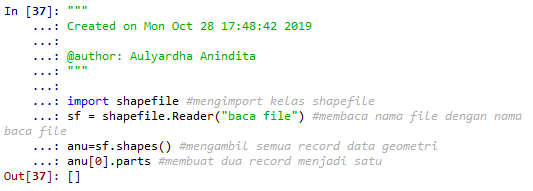
\includegraphics[width=6cm]{figures/Tugas3/1174054/no7.png}
  \centering
  \caption{Gambar Soal 7)}
 \end{figure}
 \item Nomor 8
 \lstinputlisting{src/tugas3/1174054/soal8.py}
 \begin{figure}[H]
  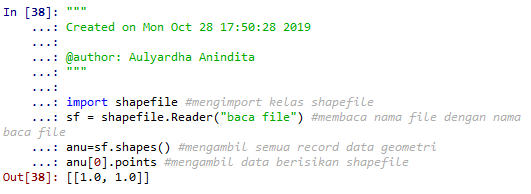
\includegraphics[width=6cm]{figures/Tugas3/1174054/no8.png}
  \centering
  \caption{Gambar Soal 8)}
 \end{figure}
 \item Nomor 9
 \lstinputlisting{src/tugas3/1174054/soal9.py}
 \begin{figure}[H]
  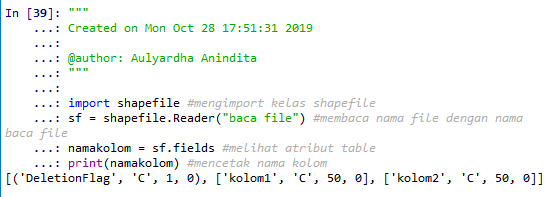
\includegraphics[width=6cm]{figures/Tugas3/1174054/no9.png}
  \centering
  \caption{Gambar Soal 9}
 \end{figure}
 \item Nomor 10
 \lstinputlisting{src/tugas3/1174054/soal10.py}
 \begin{figure}[H]
  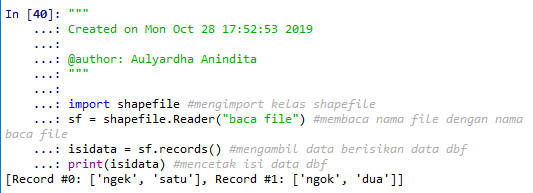
\includegraphics[width=6cm]{figures/Tugas3/1174054/no10.png}
  \centering
  \caption{Gambar Soal 10 }
 \end{figure}
 \item Nomor 11
 \lstinputlisting{src/tugas3/1174054/soal11.py}
 \begin{figure}[H]
  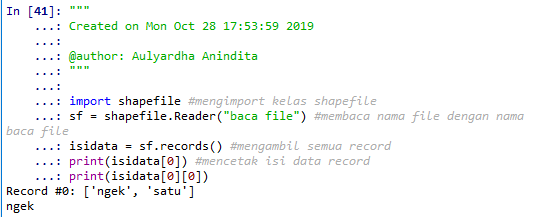
\includegraphics[width=6cm]{figures/Tugas3/1174054/no11.png}
  \centering
  \caption{Gambar Soal 11 }
 \end{figure}
\end{enumerate}
\subsection{Link}
https://youtu.be/mfib8naAOB0